% 古いコマンドやパッケージを警告
% nag - Detecting and warning about obsolete LaTeX commands
% http://www.ctan.org/tex-archive/macros/latex/contrib/nag
\RequirePackage[l2tabu, orthodox]{nag}

\documentclass[dvipdfmx]{gakugei-doctoral-course-joint-seminar}

% コメントアウト
\usepackage{comment}

% amsmath が提供しない数式環境を使用した場合に警告
% onlyamsmath
% http://www.ctan.org/tex-archive/macros/latex/contrib/onlyamsmath
\usepackage[all, warning]{onlyamsmath}

\usepackage[top=25truemm,bottom=25truemm,left=25truemm,right=25truemm]{geometry}

% 日本語のしおり文字化け対策
\begin{comment}
\ifx\kanjiskip\undefined\else
  \usepackage{atbegshi}
  \ifx\ucs\undefined
	\ifnum 42146=\euc"A4A2
	  \AtBeginShipoutFirst{\special{pdf:tounicode EUC-UCS2}}
	\else
	  \AtBeginShipoutFirst{\special{pdf:tounicode 90ms-RKSJ-UCS2}}
	\fi
  \else
	\AtBeginShipoutFirst{\special{pdf:tounicode UTF8-UCS2}}
  \fi
	\usepackage[dvipdfmx,colorlinks=false]{hyperref}
\fi
\end{comment}


\usepackage{graphicx}
\usepackage{amssymb} % 記号

%\renewcommand{\baselinestretch}{1.0} % 行送りを倍率で設定
\setlength{\baselineskip}{9pt}       % 行送りを値で設定

% 表関連
\usepackage{colortbl,array,xcolor}
\usepackage{tabularx}
\newcolumntype{C}{>{\centering}X}
\renewcommand{\tabularxcolumn}[1]{m{#1}}
\usepackage{booktabs}

% 箇条書き
\usepackage{enumitem}

\pagestyle{empty}

\title{東京学芸大学 合同ゼミナール向け \LaTeX クラスファイル}
\subtitle{題目(副題)はこの行に記入してください。副題がない場合はこの行は空白にしてください。}
\affiliation{$\circ\circ$大学 $\circ\circ$ 講座}
\grade{$\circ$年}
\keyword{\TeX, クラスファイル (重要度順に3つ程度記載してください)}
\author{佐藤 克己}

% レイアウトの確認
%\usepackage{layout}

\begin{document}

%\layout

\maketitle

\section*{章のタイトル}

研究背景や研究目的を記入してください。行数は適宜ご調節ください。

\section*{テンプレート全体についてのご案内}

\begin{itemize}
	\item 抄録はA4用紙1枚(Word or PDF形式)
	\item ページ余白は上下左右2.5cm
	\item 発表題目,学籍番号, 所属講座,学年,氏名, 配置大学をご記入ください。
	\item 内容の「見出し」は専攻ごとに形式が異なるので,適宜ご調整ください。(学校心理専攻の例:目的,方法,結果,考察,引用文献)
\end{itemize}

\section*{テンプレート全体についてのご案内}

研究結果あるいは考察について記入してください。行数は適宜ご調節ください。

\section{箇条書き}

\begin{enumerate}[labelindent=1\parindent,leftmargin=*,label=第\arabic{enumi}位.,ref=\arabic{enumi}]
		\item つぶ貝\label{enum:item1}
		\item 赤貝\label{enum:item2}
		\item ミル貝\label{enum:item3}
\end{enumerate}

\ref{enum:item1} は...

\begin{enumerate}[labelindent=2\parindent,leftmargin=*,label=第\arabic{enumi}位.,ref=お寿司 その\arabic{enumi}]
		\item マグロ\label{enum:item4}
		\item カツオ\label{enum:item5}
		\item サーモン\label{enum:item6}
\end{enumerate}

\ref{enum:item4} は...

\section{引用}

\cite{miyalab-cls}

\cite{latex2e}

\section{図}

\begin{figure}[htbp]
\centering
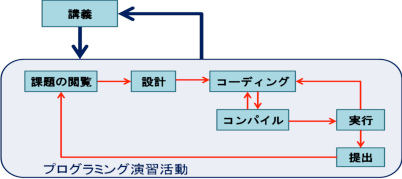
\includegraphics[width=\linewidth]{image/sample.pdf}
	\caption{サンプル画像 (PDF)}
	\label{fig:sample-pdf}
\end{figure}

\begin{figure}[htbp]
\centering
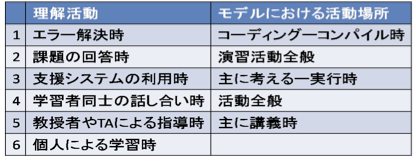
\includegraphics[width=\linewidth]{image/sample.png}
	\caption{サンプル画像 (PNG)}
	\label{fig:sample-png}
\end{figure}

画像の参照は, 図 \ref{fig:sample-pdf}, 図 \ref{fig:sample-png} のように行う。

\section{表}

表の例を表 \ref{tab:table-sample-booktabs}, \ref{tab:table-sample-rowcolor} に示す.

\begin{table}[htb]
	\caption{表の例}
	\label{tab:table-sample-booktabs}
	\begin{tabularx}{\linewidth}{CCC}
		\toprule
		\textbf{ヘッダ1} & \textbf{ヘッダ2} & \textbf{ヘッダ3}  \tabularnewline \midrule
		データ1          & データ1-1 \\
		                   データ1-2        & \checkmark        \tabularnewline \midrule
		データ2          & データ2-1 \\
		                   データ2-2        &                   \tabularnewline \midrule
		データ3          & データ3-1 \\
		                   データ3-2 \\
						   データ3-3        &                   \tabularnewline \midrule
		データ4          & データ4-1        &  \checkmark       \tabularnewline \midrule
		データ5          & データ5-1 \\ 
		                   データ5-2        &  \checkmark       \tabularnewline \bottomrule
	\end{tabularx}
\end{table}

\begin{table}[htb]
	\caption{表の例}
	\label{tab:table-sample-rowcolor}
	\begin{tabularx}{\linewidth}{|C|C|C|}
		\hline
		\rowcolor[gray]{0.8}
		\textbf{ヘッダ1} & \textbf{ヘッダ2} & \textbf{ヘッダ3}  \tabularnewline \hline
		データ1          & データ1-1 \\
		                   データ1-2        & \checkmark        \tabularnewline \hline
		データ2          & データ2-1 \\
		                   データ2-2        &                   \tabularnewline \hline
		データ3          & データ3-1 \\
		                   データ3-2 \\
						   データ3-3        &                   \tabularnewline \hline
		データ4          & データ4-1        &  \checkmark       \tabularnewline \hline
		データ5          & データ5-1 \\ 
		                   データ5-2        &  \checkmark       \tabularnewline \hline
	\end{tabularx}
\end{table}


\section{コメントアウト}

\begin{comment}
	この部分はコメントアウトされる
\end{comment}

\bibliographystyle{sieicej}

\bibliography{sample-bib}

\end{document}  
